\section{Description of the Characterization Problems}
\label{sec:AngleProbDesc}

In characterizing the $\Omega$ methods, we aim to determine in which problems
the $\Omega$-methods perform well, and then quantify that success.
First, it must be determined how effective the
$\Omega$-methods are in reducing the variance for a tally result in Monte Carlo.
This will be done by assessing and comparing the FOMs between different VR methods.
Also, the method should be investigated on a diverse set of anisotropic
problems. By constructing problems that have
different mechanisms by which the flux may be or become
anisotropic, potential strengths or weaknesses of the method can be identified.
Another desirable metric would be to quantify the method's success given the
degree of anisotropy in the problem. Recall that different
means of quantifying the flux
anisotropy were presented in Section \ref{sec:anisotropy_quant}. With a diverse
selection of characterization problems, we will obtain variation in the flux
anisotropy in each problem as well as the resultant FOMs. This will provide us
with a path forward with which to use the $\Omega$-methods in a deeper
angular-sensitivity study, which will be discussed in Section
\ref{sec:AngleResults}.

\subsection{Identification of Anisotropy-Inducing Physics}
\label{subsec:AngleProbID}

There exists a rich history of using hybrid methods in problems with strong
angular dependence, as summarized in Chapter \ref{sec:lit_review}. Angular
dependence may appear in a problem through several means--both physical and
computational.
Mosher et al. noted in their threat-detection work with ADVANTG
that problems with strongly directional sources and
problems with ``thin'' materials like air were difficult for ADVANTG to effectively
reduce the variance. The attributed this to strongly anisotropic behavior of the
importance function that were not reflected well by the scalar flux
\cite{mosher_automated_2009}. Sweezy also found that weight windows obtained
from a hybrid S$_N$ calculation were not good for a dogleg void problem,
where ray effects from the $S_N$ calculation generated poorer weight windows
than a method without ray effects \cite{sweezy_automated_2005}. Recall from
Sections \ref{sec:ContributonImportance} and \ref{sec:applicationprobs}, that ray
effects are a nonphysical effect seen in the flux solution that arise from
the angular discretization of the problem.
Ray effects are common in situations where there are strong
streaming effects or if there exists a strong source emitting particles with
long mean free paths in the material. Though they did not observe ray effects in
the importance map for the problem, Peplow et
al. also found that CADIS struggled with thin material streaming in a spherical
boat test problem \cite{peplow_consistent_2012}.

The examples of angle-dependence in problems affecting hybrid methods' success
illustrate that the flux can have anisotropy resulting from more than one
mechanism. Based on these examples, we have identified several separate
processes that affect the flux anisotropy. These processes can be grouped into
three categories: anisotropy in the flux resulting from a strongly
directional source; anisotropy resulting from strong differences between
material properties (this can be due to differences in
materials spatially and due to changes in interaction probabilities);
and anisotropy in the flux from algorithmic limitations (ray effects).
These processes have some parameter
space that overlap, so this section will continue with a brief discussion about how each
of these apply to anisotropic problems.

A strongly directional source is one that emits particles in a very small solid
angle of angle-space. The most extreme example of this would be a
monodirectional source, while an extreme opposite would be an isotropic source.
This particular anisotropy-creating process
is source-specific and does not depend on the rest of the
problem configuration. Characterization problems will have sources of both types
to ensure parameter space is covered.

% This next paragraph is maybe a little confusing and could use rewording.
The next subset of anisotropy-inducing processes are those that result form
strong differences between material properties. As noted, this can be from
the geometric configuration of the problem, or from variations in the cross
sections within a geometric location. To illustrate the differences in the way
the problem can physically induce anisotropy in the flux, several simple thought
experiments will be presented. Consider first the extreme example of material
A which has some low absorption probability,
and material B which is a pure absorber. Only
particles that travel through material A will eventually reach the tally
location. This is an example of a type of problem with strong material
heterogeneity. In constructing a set of characterization problems, creating channels
through which particles will preferentially travel will induce anisotropy in the
flux. These types of flow paths are also of interest in shielding application
problems, and were discussed at length in Section
\ref{sec:ContributonImportance}. In this type of problem, material A can either
have a low scattering probability (airlike), or it can be highly scattering. In
scattering events, neutral particles can either lose very little energy with a high Z
material, like lead, or they can lose a lot of energy with a low Z material.
These will be considered separately, because the energy spectrum of the
particles affects the particle's interaction probability.
Consider another example of an isotropic
point source immersed in a pure thin material. Because particles have a very low
probability of interaction in the material, they will travel almost uniformly
outwards away from the point source. At some distance from the point source, the
majority of the
particles in a cell will be traveling in the same direction. This is an example
of a problem with streaming paths.
To summarize, we have identified several
sub-distinctions of this type of effect: regions with streaming where particles
far from the source are primarily monodirectional, regions
that are highly scattering where particles have a preferential flowpath through
one material and are downscattered in energy, and regions with strong
material heterogeneity where particles have preferential flowpaths but are not
necessarily downscattered in energy. It should be noted that while streaming and
scattering problems will almost always be subsets of problems with material
homogeneity, it is possible to have a highly scattering or a streaming problem
without material heterogeneity.

The last factor that can influence anisotropy in the flux solution is ray
effects. While ray effects are a result of anisotropy in the flux solution, this
is a nonphysical effect and can actually affect variance reduction
performance. In the case of ray effects, we aim to see if the
$\Omega$-methods are more robust in avoiding them in generating VR parameters.
Because ray effects are primarily seen in large regions with low interaction
probabilities, some of the characterization problems will need to
incorporate these regions into their geometries.

In this subsection, four primary physical mechanisms by which the flux may
be anisotropic were identified. These are streaming paths, problems with high
scattering effects, problems with high material heterogeneity (specifically with
materials with strong differences in scattering and absorption probabilities),
and problems with monodirectional sources. As described in the preceding
paragraphs, a few of these mechanisms may overlap
with one another. They comprise a large subset of flux
anisotropy-inducing physics, and combined with different geometric arrangements
in sample problems a diverse group anisotropic problems can be formulated. These
problems can then be used to characterize the $\Omega$-methods.

\subsection{Problem Specifications}
\label{subsec:ProbSpecs}

With the anisotropy-inducing physics described in Section
\ref{subsec:AngleProbID}, a set of characterization problems that have
different combinations of each of these effects can be conceptualized. With
different anisotropy-inducing physics in the system, these problems will provide
an overview of how the $\Omega$-methods perform in an assortment of anisotropic
problems. The primary anisotropy-inducing features identified are: streaming
paths, material heterogeneity, materials with highly differing scattering
probabilities, and monodirectional sources. As previously described, these fall
into two broad categories: anisotropy caused by the problem materials and
geometry, and anisotropy caused by the source definition. In the next few
paragraphs, each problem will be described and will be accompanied by
a justification for which
anisotropy-inducing physics is in each problem. A summary of which physics are
in each problem is provided in Table \ref{tab:probphysics}.

\subsubsection*{Experimental Beamline}

\begin{figure}[h!]
  \centering
  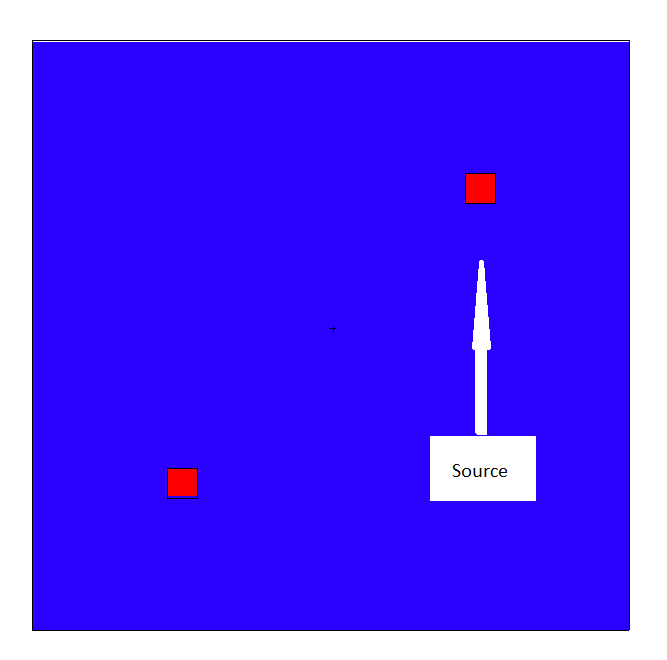
\includegraphics[height=8cm]{./chapters/characterization_probs/figures/geometries/beam.png}
  \caption[Nuclear physics experimental beamline.]{Nuclear physics experimental beamline.}
  \label{fig:beamgeom}
\end{figure}

The experimental beamline illustrated in Fig. \ref{fig:beamgeom} is an
application problem that will have very strong angular dependence in the flux. The
facility is primarily air, with two sodium iodine detectors in the room. The
beamline--a monodirectional source--is aimed towards the first detector, and
the response in the second detector (at a 45\degree angle
relative to the beamline) is to be optimized with CADIS. In this problem, we
expect anisotropy to occur in the flux from both the monodirectional source and
the very strong streaming effects that will occur from the low-density air.
These streaming effects will also cause ray effects to appear in the
deterministic solutions. This
problem will be very high energy, with little opportunity for particles to
slow down from moderating materials. The only moderating materials in the
problem are located in the detectors, and as a result it is the only problem
that has strong streaming effects but does not have material heterogeneity.

\subsubsection*{Labyrinths}

The labyrinth problems have isotropic point sources on the left hand side of the
problem emitting a watt spectrum of
neutrons approximating the energy spectrum emitted by that of $^{235}$U fission.
On the right hand side of the problem there is a NaI detector recording the flux.
They are both composed of a concrete maze with an air channel through the maze, and
then open air channels at either end of the channels. The first variant of the
labyrinth has a single turn, as illustrated in Figure \ref{fig:maze2geom}, and
the second labyrinth has multiple turns, as illustrated in Figure
\ref{fig:maze1geom}. These problems are both
likely to have ray effects in the air region near the forward source. However,
because far more scattering events will be required for a particle to exit the
channel in the multi-turn maze, ray effects will likely be less prominent in the
air region near the detector of that variant problem than it is in the single
turn maze. Both problems have strong
differences in interaction probabilities between the air and the concrete,
thus they will have material heterogeneity. Further, because the concrete is
composed of several lighter-mass elements, these will also be highly scattering.

\begin{figure}[h!]
  \centering
  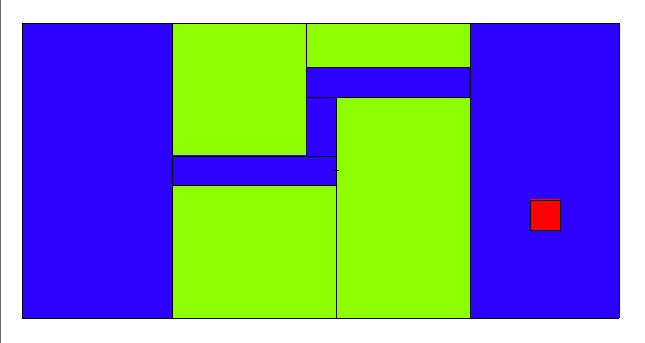
\includegraphics[width=10cm]{./chapters/characterization_probs/figures/geometries/maze2.png}
  \caption[Single turn labyrinth geometry.]{Single turn labyrinth geometry.}
  \label{fig:maze2geom}
\end{figure}

\begin{figure}[h!]
  \centering
  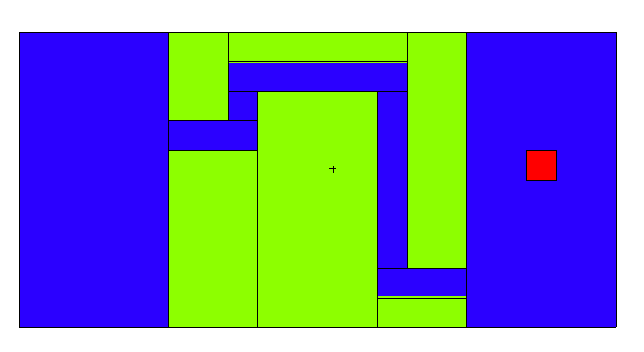
\includegraphics[width=10cm]{./chapters/characterization_probs/figures/geometries/maze1.png}
  \caption[Multi-turn labyrinth geometry.]{Multi-turn labyrinth geometry.}
  \label{fig:maze1geom}
\end{figure}

\subsubsection*{Steel beam in Concrete}

\begin{figure}[h!]
  \centering
  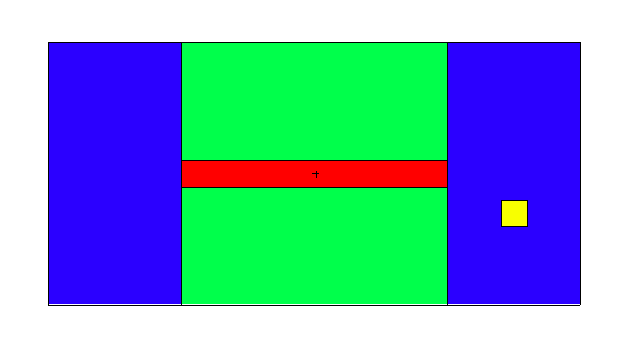
\includegraphics[width=12cm]{./chapters/characterization_probs/figures/geometries/prob-1.png}
  \caption[Steel plate embedded in concrete.]{Steel plate embedded in concrete.}
  \label{fig:prob1geom}
\end{figure}

Figure \ref{fig:prob1geom} is a variant problem with a steel beam embedded in
concrete. A NaI detector is located on the right hand side of the problem to
record the response in CADIS problems. The source is a 80x80cm sheet pointed in
towards the steel structure in the $+x$ direction emitting 10MeV neutrons.
Because the particles have preferential flow through the steel but do do not
have long streaming paths, this problem has material heterogeneity and will be
highly scattering, but it will not have streaming paths in the shielding region.
Further, because the source is emitted from a thin plate in $+x$, it is
monodirectional. This problem may have some ray effects occurring from
backscattering off of the steel and concrete in the left side air region, and it
may also have some exiting the beam on the right hand side. However, because
significantly more scattering will happen in the concrete, the ray effects on
the right hand side will be less pronounced than in the low-density maze exits.

\subsubsection*{U-shaped corridor}

\begin{figure}[h!]
  \centering
  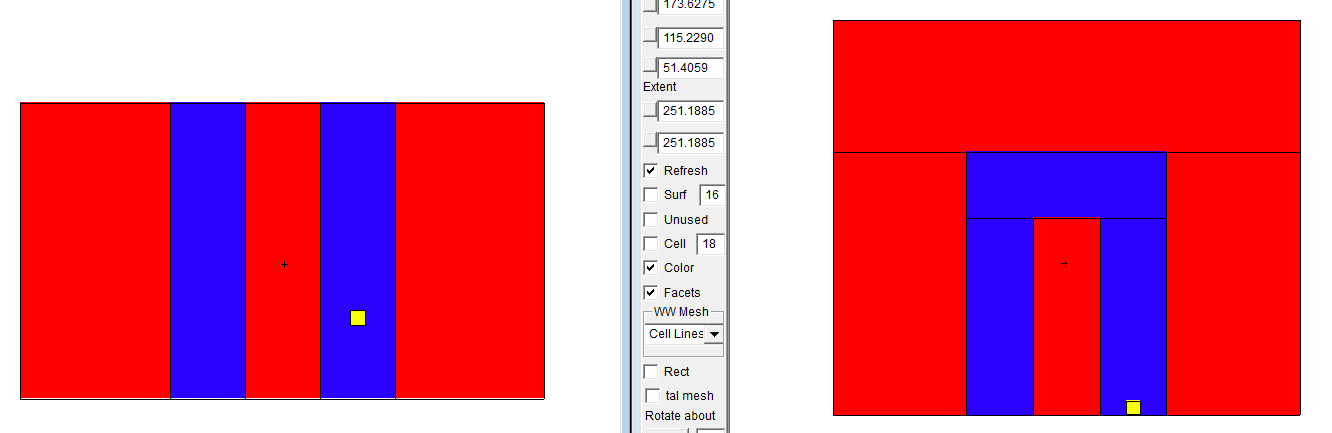
\includegraphics[width=15cm]{./chapters/characterization_probs/figures/geometries/prob-2.png}
  \caption[U-shaped corridor in concrete]{U-shaped corridor in concrete.}
  \label{fig:prob2geom}
\end{figure}

The u-shaped corridor illustrated in Figure \ref{fig:prob2geom} is somewhat
similar to the maze variants from Figs. \ref{fig:maze2geom} and
\ref{fig:maze1geom}. On the left-hand side of the corridor there is a point source
emitting a watt specturum of $^{235}$U neutrons. The right leg of the corridor
has a NaI detector. Without the large air voids in the labyrinth variants, the
U-shaped corridor will have
less-prominent ray effects. The heterogeneity between
the air and concrete will preferentially transport particles through the air,
and particles interacting with the concrete will downscatter in energy. This

\subsubsection*{Concrete shielding with rebar}

\begin{figure}[h!]
  \centering
  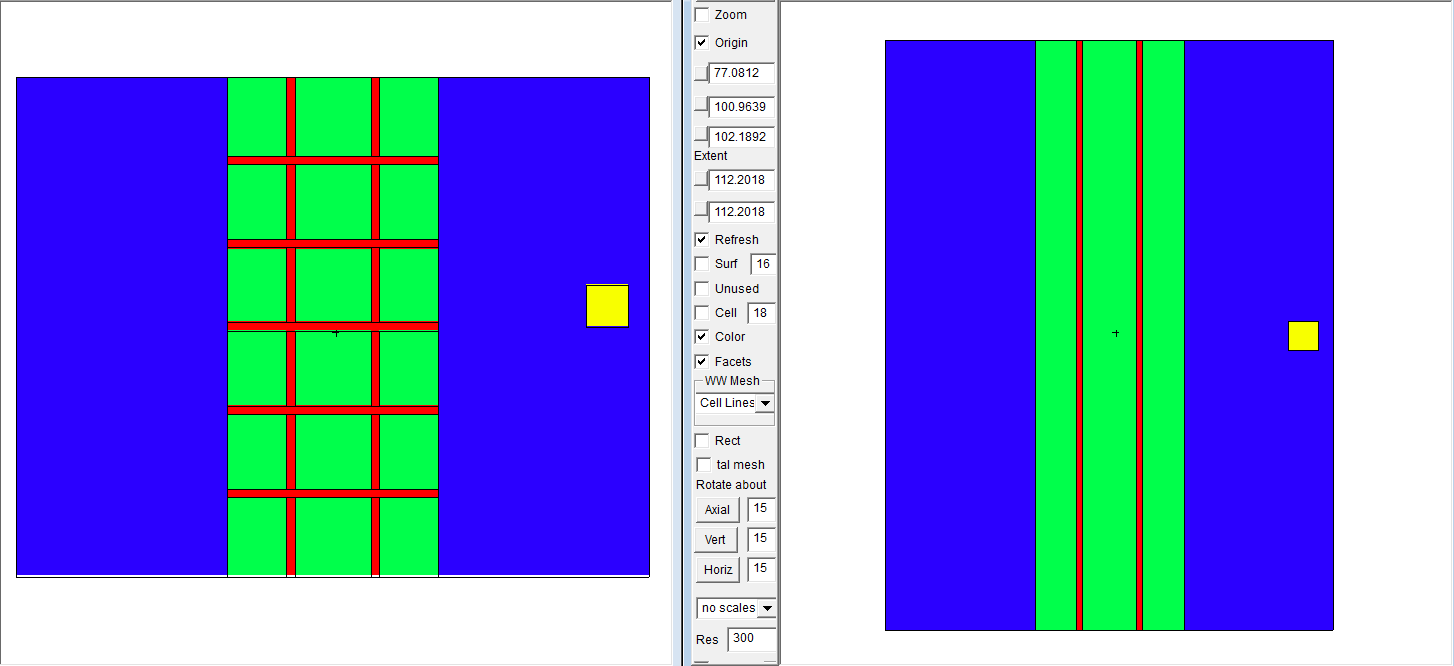
\includegraphics[width=15cm]{./chapters/characterization_probs/figures/geometries/prob-4.png}
  \caption[Concrete shielding with rebar]{Concrete shielding with rebar.}
  \label{fig:prob4geom}
\end{figure}

The shielding material illustrated in Figure \ref{fig:prob4geom} is built off of
the steel structural beam problem in Figure \ref{fig:prob1geom}. However, this is a more
realistic illustration of rebar in concrete. In this problem, a NaI detector is
used to measure the response on the right hand side of the problem in yellow.
The source is both space- and energy-dependent, emitting a watts spectrum of
neutrons characteristic of 235U fission, and is distributed in a 100x160cm plate
on the left hand side of the problem. The source is monodirectional in $+x$.
The two images provided show
different xy-plane cutaways of the shielding, with steel rebar running through
the concrete in different directions. This problem should have angular
dependence, but preferential flowpaths through the concrete are not directed
towards the detector location on the other side of the shielding in some of the
rebar. This problem has material heterogeneity both in the concrete and between
the concrete and air. This problem is highly scattering from the concrete, and
is unlikely to have ray effects without a strong single preferential flowpath
through the shield.

\subsubsection*{Nuclear medicine therapy room}

\begin{figure}[h!]
  \centering
  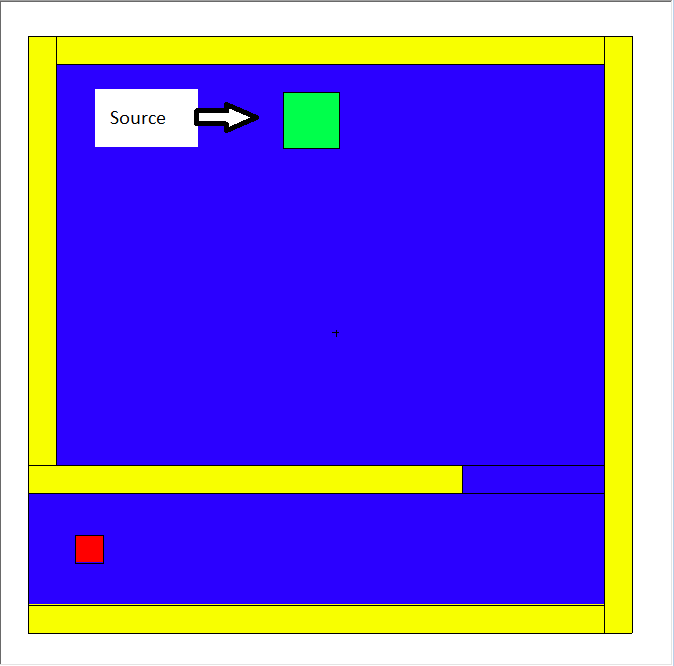
\includegraphics[height=8cm]{./chapters/characterization_probs/figures/geometries/therapy-room.png}
  \caption[Nuclear medicine therapy room.]{Therapy room geometry.}
  \label{fig:therapygeom}
\end{figure}

A small application problem relevant to the interests of this project is the
therapy room illustrated in Figure \ref{fig:therapygeom}. This room has concrete
walls, a water-based phantom that is being irradiated by a monodirectional
source in the room, and a hallway where a therapy technician might walk. In a
CADIS-run of this problem, we seek to calculate the response in the
technician in the hallway from particles that are not absorbed by the patient in
the room. Because this problem is primarily air with concrete
borders, it will have strong streaming effects in the air. Particles that do
make it to the technician will be produced by emission from the patient in the
room, by scattering off of the problem air, or by scattering off of the problem
walls. Because of the high fraction of air in this problem, we also anticipate
ray effects to occur. While there will be scattering in this problem, it will
not be as strong of an effect as other characterization problems.

Now that the broad subset of characterization problems have been described,
the physics that each contains is summarized in Table \ref{tab:probphysics}.
Upon glancing at the table, one may see that it can be difficult to separate
out one physical mechanism from another when constructing problems. This is
especially true in generating a problem that has ray effects without streaming
paths, and in constructing a highly scattering problem that has preferential
flow paths but does not have material heterogeneity. This is a
deficiency of the characterization problem construction, and is certainly an
area that may be improved upon in future work.

\begin{table}[h!]
  \centering
  \begin{tabular}{l|C{2cm}C{2cm}C{2cm}C{2cm}C{2cm}}
% \begin{tabular}{l|ccccc}
\toprule
\multirow{2}{*}{Problem Name} &  \multicolumn{4}{c}{Problem Coverage} \\
{} &  Streaming Paths & Highly Scattering & Material Heterogeneity &
Monodirectional Source & Ray \newline Effects \\
\midrule
Beamline              & x &   &   & x & x \\
Maze variants         &   &   &   &   &   \\
\textit{Single turn}  & x & x & x &   & x \\
\textit{Multi-turn}   & x & x & x &   & x \\
Steel plate           &   & x & x & x & x$^{\dagger}$  \\
U-shaped corridor     & x & x & x &   &   \\
Shielding with rebar  &   & x & x & x &   \\
Therapy Room          & x &   & x & x & x \\
\bottomrule
\end{tabular}
\begin{flushleft}
\footnotesize{
  $^{\dagger}$ May have ray effects in low density region exiting the metal
  plate, but effects will be less pronounced than other problems.
}
\end{flushleft}

  \caption[Anisotropy-inducing physics of each of the characterization problems.]
  {Anisotropy-inducing physics of each of the characterization problems.
  Each identified anisotropy-inducing physical metric is used in different
  combinations for the characterization problems. This will help to aid in
  extrapolating to which real problems the $\Omega$-methods may be applied.}
  \label{tab:probphysics}
\end{table}
% maybe it would be worthwhile to add a table of source definitions between each
% of the char problems. Some of them are monoenergetic, some are
% monodirectional, and some are monospatial(?) (point sources). A table would be
% a good way to summarize this information.

\subsection{Introduction the Presented Data}
\label{subsec:resultsintro}

The results for the characterization problems and the subsequent angle
sensitivity study will have a substantive amount of data. Only the most
pertinent fraction of the available data will be presented with each problem.
A more extensive set of data is available in Appendix \ref{ch:extended}. The
characterization problems will have extended results in Section
\ref{sec:extendedcharprobs} and the angle sensitivity study will be in
\ref{sec:extendedangle}. To provide a more tangible approach to the theoretical success
metrics that were presented in Section \ref{sec:successmetrics}, the next few
paragraphs will present the types and variety of data that may be presented in
Sections \ref{sec:CharResults}, \ref{sec:AngleResults},
\ref{sec:extendedcharprobs} and \ref{sec:extendedangle}. This will be
accompanied by some discussion into the factors influencing these metrics, when
relevant.

In Section \ref{sec:FOMvariants} several variants of the Figure of Merit were
presented as quantifications of method success. In the

\begin{table}[h!]
  \centering
  \begin{tabular}{l|m{3.5cm}m{3.5cm}m{3.5cm}}
\toprule
{} &   \multicolumn{2}{c}{CADIS or CADIS-$\Omega$}   & analog \\
{FOM Variant} &   MC \eqref{eq:FOMMC} & MC$_{hybrid}$ \eqref{eq:FOMHybrid} &  MC \\
\midrule
tally avg \eqref{eq:FOMavg}  &  FOM$_{avg,MC}$ &   FOM$_{avg,hybrid}$   & FOM$_{avg,MC}$   \\
max RE  \eqref{eq:FOMmax}    &  FOM$_{max,MC}$  &   FOM$_{max,hybrid}$  &  FOM$_{min,MC}$ \\
min RE      &   FOM$_{min,MC}$  &   FOM$_{min,hybrid}$   &  FOM$_{min,MC}$ \\
time (mins) & T$_{MC}$ & T$_{hybrid}$ \eqref{eq:hybridtime} &  T$_{MC}$ \\
\bottomrule
\end{tabular}

  \caption[Table of FOM variants used to measure $\Omega$ performance.]{
  Table of FOM variants used to measure $\Omega$ performance. Relevant Eqs. can
  be found in Section \ref{sec:FOMvariants} and are referenced in the table in
  brackets.}
  \label{tab:fom_defaults}
\end{table}


